\documentclass[tikz,border=3.14mm]{standalone}
\usetikzlibrary{positioning,chains,fit}
\usepackage{xcolor}
\colorlet{myred}{red!80!black}
\colorlet{myblue}{blue!80!black}
\colorlet{mybluee}{myblue!80!black}
\colorlet{mygreen}{green!60!black}
\colorlet{myorange}{orange!70!red!60!black}
\colorlet{mydarkred}{red!30!black}
\colorlet{mydarkblue}{blue!40!black}
\colorlet{mydarkgreen}{green!30!black}
\begin{document}
\begin{tikzpicture}[
    >=latex,
    node/.style={thick,minimum size=22,inner sep=0.5,outer sep=0.6, rounded corners=0.2cm},
    node in/.style={node,green!20!black,draw=mygreen!30!black,fill=mygreen!25},
    node hidden/.style={node,blue!20!black,draw=myblue!30!black,fill=myblue!20},
    node out/.style={node,red!20!black,draw=myred!30!black,fill=myred!20},
    connect/.style={thick,mydarkblue},
    connect arrow/.style={->,thick,mydarkblue,shorten <=0.5,shorten >=1},
    block/.style={rectangle, draw, minimum width=2cm, minimum height=1cm, align=center},
]
% GoogLeNet placeholder
\node[inner sep=0, outer sep=0] (googlenet) at (0,0) {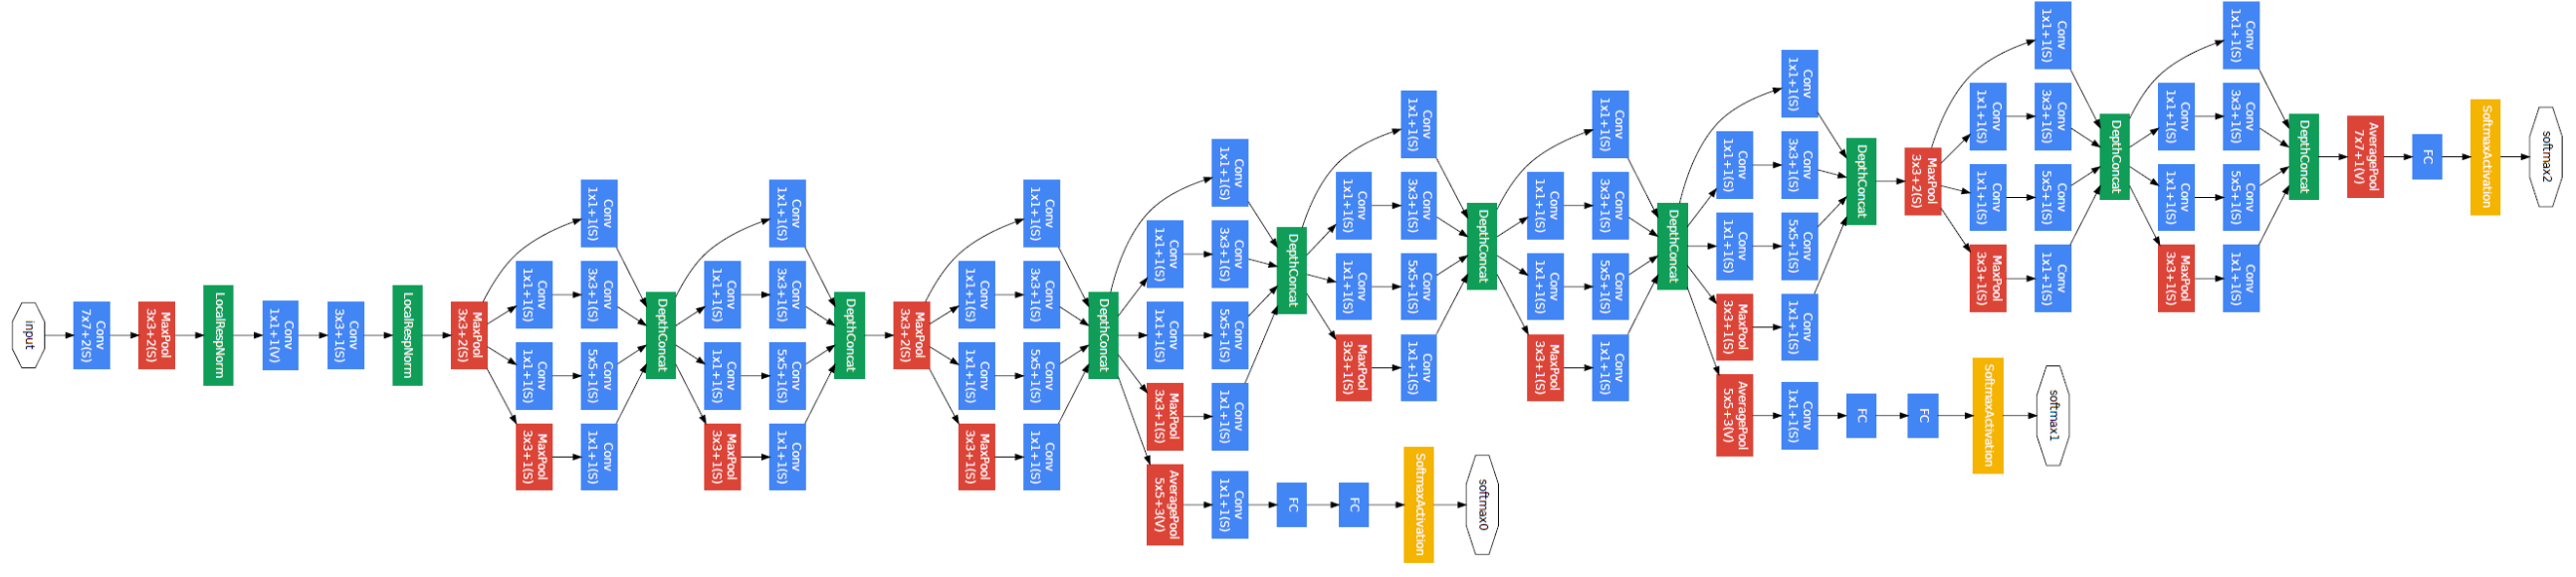
\includegraphics[angle=90,origin=c,width=2cm,height=5cm]{tikz/chapter5 - GoogleNet.png}};
\node[fit=(googlenet), draw] {};
\node[below=0.7cm of googlenet, node, orange!20!black,draw=myorange!20!black,fill=myorange!25, minimum width=1.2cm] (image) {image};
\node[xshift=2.5cm, block, node hidden, minimum width=1.4cm] (lstmBegin) {LSTM};
\node[right=0.7cm of lstmBegin, block, node hidden, minimum width=1.4cm] (lstm1) {LSTM};
\node[block, above=0.8cm of lstm1, node out] (p1) {$p_1$};
\node[block, above=0.8cm of p1, node out, minimum width=1.7cm] (log1) {$\log p_1(S_1)$};
\node[block, below=0.8cm of lstm1, node in, minimum width=1cm] (w1) {$W_e S_0$};
\node[block, below=0.8cm of w1, node in] (s1) {$S_0$};
\node[right=0.7cm of lstm1, block, node hidden, minimum width=1.4cm] (lstm2) {LSTM};
\node[block, above=0.8cm of lstm2, node out] (p2) {$p_2$};
\node[block, above=0.8cm of p2, node out, minimum width=1.7cm] (log2) {$\log p_2(S_2)$};
\node[block, below=0.8cm of lstm2, node in, minimum width=1cm] (w2) {$W_e S_1$};
\node[block, below=0.8cm of w2, node in] (s2) {$S_1$};

% Add the final LSTM block
\node[right=1.4cm of lstm2, block, node hidden, minimum width=1.4cm] (lstmN) {LSTM};
\node[block, above=0.8cm of lstmN, node out] (pN) {$p_N$};
\node[block, above=0.8cm of pN, node out, minimum width=1.7cm] (logN) {$\log p_N(S_N)$};
\node[block, below=0.8cm of lstmN, node in, minimum width=1cm] (wN) {$W_e S_{N-1}$};
\node[block, below=0.8cm of wN, node in] (sN) {$S_{N-1}$};

% Add connecting arrows
\draw[connect arrow] (image) -- (googlenet);
\draw[connect arrow] (googlenet) -- (lstmBegin);
\draw[connect arrow] (lstmBegin) -- (lstm1);
\draw[connect arrow] (lstm1) -- (lstm2);
\draw[connect arrow] (lstm2) -- node[above, midway] {\ldots} (lstmN);

\draw[connect arrow] (lstm1) -- (p1);
\draw[connect arrow] (p1) -- (log1);
\draw[connect arrow] (w1) -- (lstm1);
\draw[connect arrow] (s1) -- (w1);

\draw[connect arrow] (lstm2) -- (p2);
\draw[connect arrow] (p2) -- (log2);
\draw[connect arrow] (w2) -- (lstm2);
\draw[connect arrow] (s2) -- (w2);

\draw[connect arrow] (lstmN) -- (pN);
\draw[connect arrow] (pN) -- (logN);
\draw[connect arrow] (wN) -- (lstmN);
\draw[connect arrow] (sN) -- (wN);

\end{tikzpicture}
\end{document}